\documentclass[]{foi} % zakomentirati za pisanje rada na engleskom jeziku
% \documentclass[english]{foi} % odkomentirati za pisanje rada na engleskom jeziku
\usepackage[utf8]{inputenc}
\usepackage{lipsum}

\vrstaRada{\projekt \\\MakeLowercase{\href{https://www.overleaf.com/read/vvppvhrhcrkk}{(\textit{\underline{Overleaf.com}})}}} % \diplomski
% \zavrsni ili \diplomski ili \seminar ili \projekt

\title{Agenti kao konačni automati za pregled vijesti}
\predmet{\predmetVAS}
% ostaviti prazno ako \vrstaRada nije \projekt ili \seminar
% \predmetBP ili \predmetDP ili \predmetTBP ili \predmetVAS

\author{{\href{https://github.com/jantolos/MASproject_2022}{\textit{\underline{Jerry John Antolos}}}}} % ime i prezime studenta/studentice
\spolStudenta{\musko} % \zensko ili \musko

\mentor{Bogdan Okreša Đurić} % ime i prezime mentora
\spolMentora{\musko} % \zensko ili \musko
\titulaProfesora{dr. sc.}
% HR: dr. sc.  / doc. dr. sc. / izv. prof. dr. sc. / prof. dr. sc. 
% EN: -prazno- / Asst. Prof.  / Assoc. Prof.       / Full Prof.

\godina{2022}
\mjesec{srpanj} % mjesec obrane rada ili projekta

\indeks{0016120073} % broj indeksa ili JMBAG

\smjer{Baze podataka i baze znanja}
% (ili:
%     Informacijski sustavi, 
%     Poslovni sustavi, 
%     Ekonomika poduzetništva, 
%     Primjena informacijske tehnologije u poslovanju, 
%     Informacijsko i programsko inženjerstvo, 
%     Baze podataka i baze znanja, 
%     Organizacija poslovnih sustava, 
%     Informatika u obrazovanju
% )


\sazetak{Cilj ovog projektnog zadatka bio je napraviti aplikaciju pomoću višeagentnog sustava koja će iz različitih javno dostupnih resursa dohvaćati vijesti i prikazivati ih korisniku. Razmišljajući o UX  korisniku se omogućilo filtriranje vijesti prema ključnim riječima.}

\kljucneRijeci{SPADE; konačni automat; višeagentni sustav; pretraživanje vijesti;}



\begin{document}

\maketitle

\tableofcontents

\makeatletter \def\@dotsep{4.5} \makeatother
\pagestyle{plain}



\chapter{Uvod}

\chapter{Teorijski uvod}
U sklopu predmeta Višeagentni sustavi na diplomskom studiju Baze podataka i baze znanja Fakulteta organizacije i informatike Sveučilišta u Zagrebu potrebno je bilo osmisliti, implementirati i dokumentirati zadatak na samostalno odabranu temu. Odabrao sam temu "Agenti kao konačni automati za pregled vijesti". Između ostalog zadatak je bio da se u sklopu teme implementiramo višeagentnog sustava koja će iz javno dostupnih resursa dohvaćati vijesti i prikazivati ih korisniku.

Na početku je svakako dobro postaviti pitanje ima li projekt smisla odnosno pitanje možemo malo proširiti pa postaviti ga na drugačiji način ima li smisla razvijati agente za internetske aplikacije i kakve su koristi od njih. Pa upravo na ovo pitanje daju odgovor autori Enembreck, Barthès i Ávila u svom radu \cite{10.1007/978-3-540-30104-2_7} Oni kažu kako upravo korištenje višeagenatnih sustava može imati brojne prednosti kao što su skalabilnost, stabilnost ili balansiranje opterećenja.

Kada govorimo o skalabilnosti tada mislimo na to da sustav možemo ažurirati ili proširiti bez utjecaja na njegove ostale funkcije budući da su agenti neovisni sustavi. Pojam stabilnosti nam govori o tome da kad god se neki agent sruši uvijek drugi agent može koordinirati distribuciju usluga.

\section{SPADE}

SPADE je skračenica koja dolazi iz engleskog govornog područja, a znači Smart Python multi-Agent Development Environment. Riječ je o platformi koja se temelji na XAMPP tehnologiji i pisana je u programskom jeziku Python. SPADE je platforma koja trenutno podržava isključivo Python programski jezik odnosno SPADE je Python modul za razvoj softverskih agenata. \cite{Spade}
Agenti mogu imati nekoliko ponašanja koji se mogu odvijati u isto vrijeme. Riječ je o sljedećim ponašanjima:

\begin{itemize}
  \item Cyclic
  \item Periodic 
  \item Time-Out
  \item One-shot
  \item Finite State Machine 
  \item Event Behaviour
\end{itemize}

\section{Agent kao konačni automat}
Kako bi uopće počeli implementaciju agenta kao konačnog automata moramo znati zapravo što je konačni automat kao takav. Prema definiciji konačnog automata koju možemo pročitati na Wikipediji konačni automat je diskretni matematički model koji se sastoji od konačnog broja stanja, prijelaza između tih stanja, i akcija koje obavlja. \cite{konacniAutomat} 

Dok ako bi htjeli definirati agente kao konačne automate možemo se poslužiti i definicijom koju smo odradili na predavanjima. Ova definicija nam detaljizira agente kao konačne automate, a glasi:

Konačni automat je šestorka (\(\Sigma, \Gamma, S, S_0, \delta, \omega\)) pri čemu je:
\begin{itemize}
  \item \(\Sigma\) ulazna abeceda (konačni neprazni skup simbola)
  \item \(\Gamma\) izlazna abeceda (konačni neprazni skup simbola)
  \item \(S\) konačni neprazni skup stanja
  \item \(S_0\) početno stanje (\(S_0 \in\) S)
  \item \(\delta\) funkcija prijelaza \( \delta : S \times \Sigma \rightarrow S\)
  \item \(\omega\) izlazna funkcija \( \omega : S \times \Sigma \rightarrow \Gamma\)
\end{itemize}\cite{agentiKonacniAutomati}

\chapter{Instalacija potrebnih paketa}
Na samom početku potrebno je postaviti razvojnu okolinu i instalirati potrebne pakete kako bi uspješno mogli razviti programski proizvod. U sljedećim poglavljima imati ćemo priliku vidjeti koji su nam sve paketi potrebni i kako ih instalirati na naš uređaj.
\section{Instalacija paketa \textit{spade}}
Za početak krenuti ćemo s platformom SPADE. Kao i što smo naveli SPADE je platforma za razvoj višeagentnih sustava u programskom jeziku Python. Kako bi ju instalirali potrebno je pokrenuti naredbu: \begin{verbatim}.\pip install spade\end{verbatim} Nakon što smo pokrenuli naredbu instalacija će se pokrenuti a po završetku instalacije ispis na ekranu konzole bi trebao izgledati kao na slici 1.

\begin{figure}[h!]
    \centering
    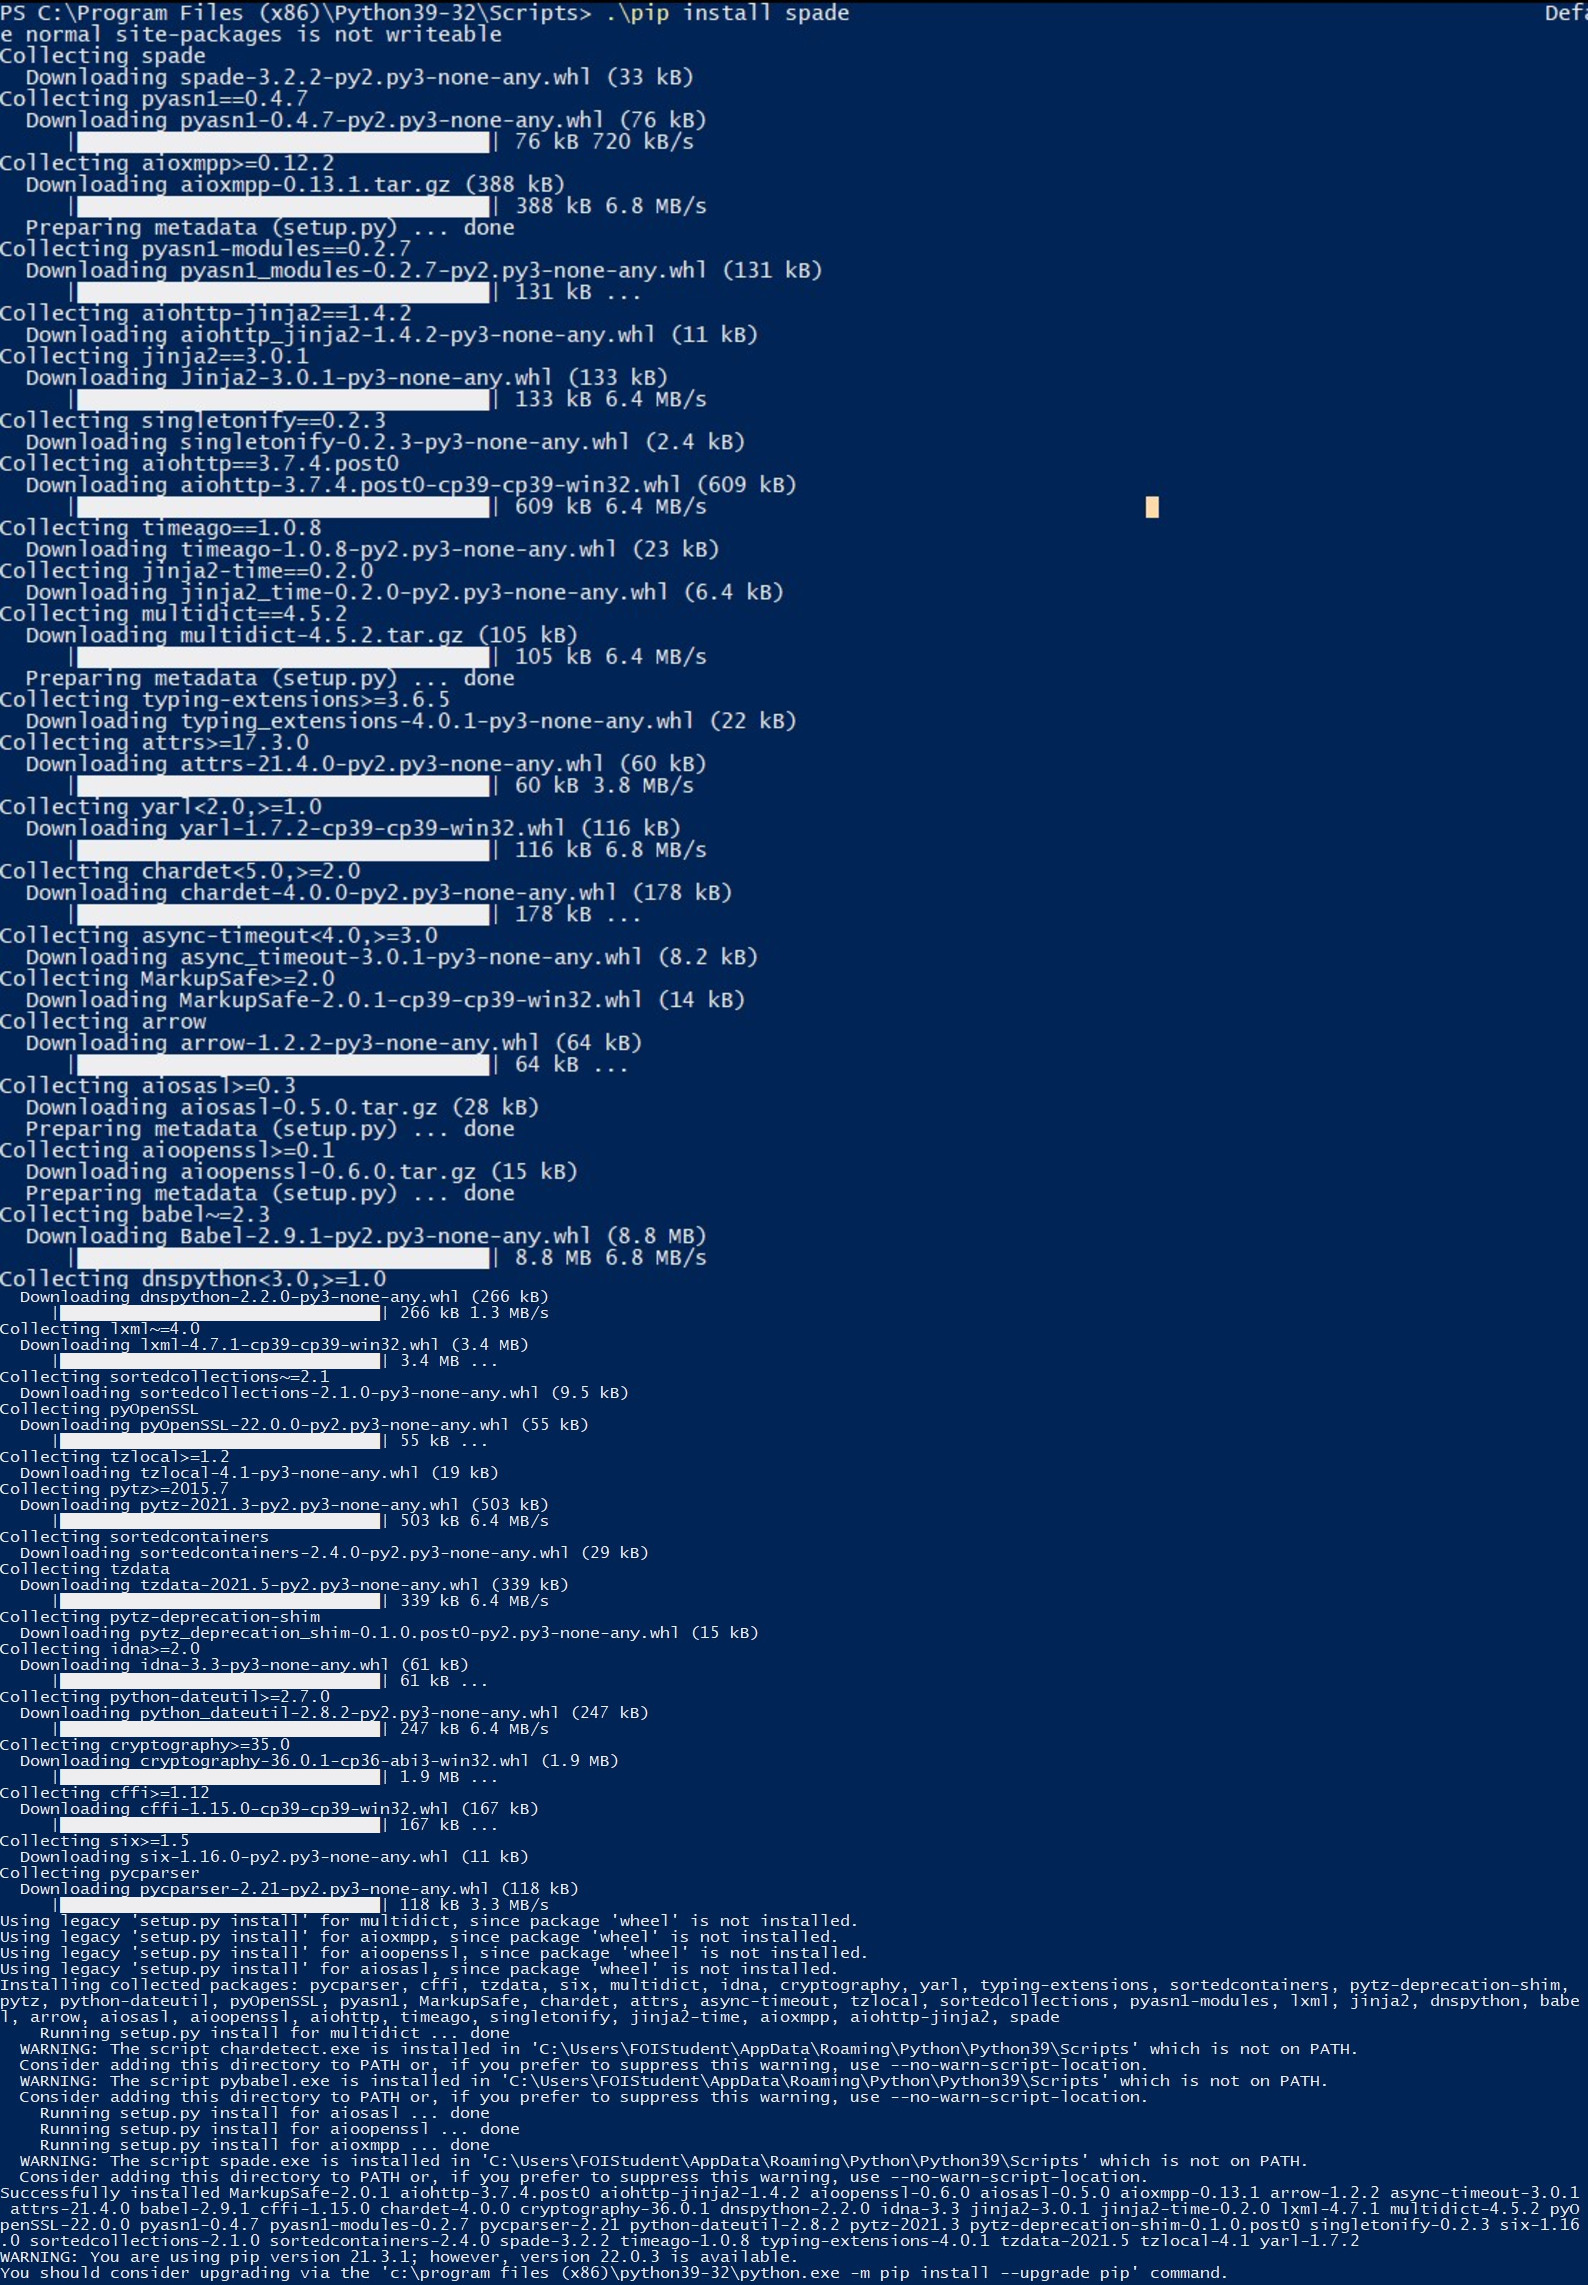
\includegraphics[width=0.6\textwidth]{slike/spade-install.jpg}
    \caption{Instalacija paketa \textit{spade} (Izvor: \citeauthor{ispisInstalacijeSpade} \citeyear{ispisInstalacijeSpade})}
    \label{fig:instalacijaSPADE}
\end{figure}

Sada je uspješno instaliran SPADE te možemo prijeći na sljedeći korak instalacije. Kao sljedeći korak, kako bi mogli raditi s HTTP zahtjevima, instalirati ćemo paket \textit{requests}.

\section{Instalacija paketa \textit{requests}}
Paket \textit{requests} je biblioteka koja je razvijena s ciljem da ljudima koji ju koriste omogući jednostavniji rad s HTTP zahtjevima. Upravo ovaj razlog je i bio krucijalan da se odlučim za korištenje ovog paketa. Proces instalacije ovog paketa ne razlikuje se od instalacije bilo kojeg drugog paketa u Pythonu. Dakle, kako bi pokrenuli instalaciju ovog paketa dovoljno je pokrenuti sljedeću naredbu:\begin{verbatim}.\pip install requests\end{verbatim} Po završetku instalacije u konzoli ispisati će se kako slijedi

\begin{figure}[h!]
    \centering
    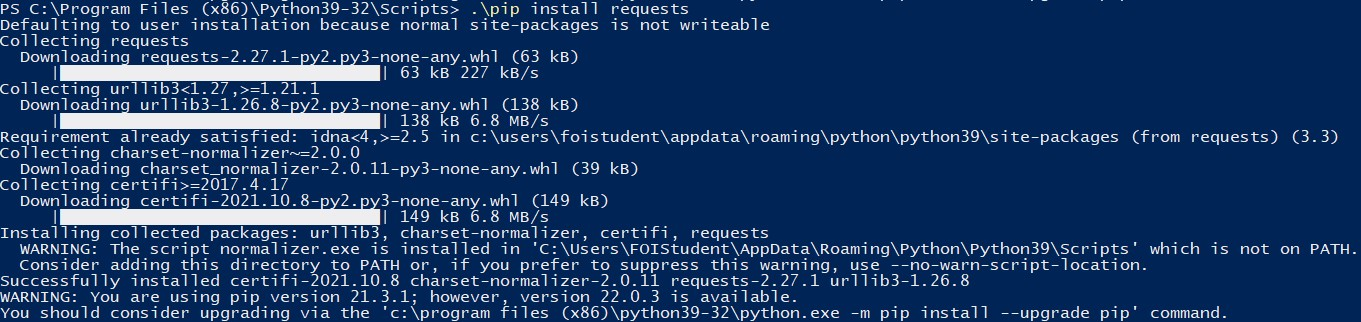
\includegraphics[width=1.0\textwidth]{slike/requests-install.jpg}
    \caption{Instalacija paketa \textit{requests} (Izvor: \citeauthor{ispisInstalacijeRequests}, \citeyear{ispisInstalacijeRequests})}
    \label{fig:instalacijaRequests}
\end{figure}

Nakon uspješne instalacije paketa \textit{requests} skoro pa imamo sve potrebno da započenemo rad na sustavu. Namjerno kažem skoro sve jer nedostaje glavni dio - paket koji će nam pomoći da izvučemo podatke iz HTML datoteke. Kako bi ovo učnili potreban nam je paket \textit{beautifulsoup4}.

\section{Instalacija paketa \textit{beautifulsoup4}}
\textit{beautifulsoup4} je paket koji služi za izvlačenje podataka zarobljenih između HTML oznaka u HTML dokumentu. Ovaj paket je važan kako bi mogli izvući novosti s dostupnih web izvora i prikazati ga korisnicima u sklopu našeg sustava. Kao i dosada pokrenuti ćemo instalaciju unosom sljedeće naredbe:\begin{verbatim}.\pip install beautifulsoup4\end{verbatim}

\begin{figure}[h!]
    \centering
    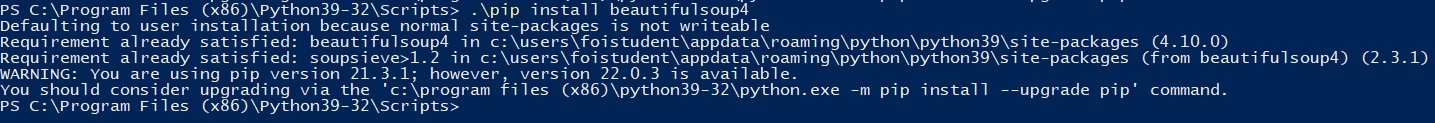
\includegraphics[width=1.0\textwidth]{slike/beautifulsoup4-install.jpg}
    \caption{Instalacija paketa \textit{beautifulsoup4} (Izvor: \citeauthor{ispisInstalacijeBeautifulsoup4}, \citeyear{ispisInstalacijeBeautifulsoup4})}
    \label{fig:instalacijaBeautifulSoup4}
\end{figure}

Ako je paket već instaliran na računalu na kojem radimo onda će ispis u konzoli biti istovjetan ispisu prikazanom na slici 3.

Ovim posljednjim korakom instalacije paketa završili smo pripremu za početak razvoja višeagentnog sustava. Sada možemo pokrenuti Python IDLE razvojno okruženje i početi s razvojem.Nakon što pokrenemo razvojno okruženje i otvorimo novu datoteku za pisanje programskog koda naše razvojno okruženje izgleda kao na slici 4.

\begin{figure}[h!]
    \centering
    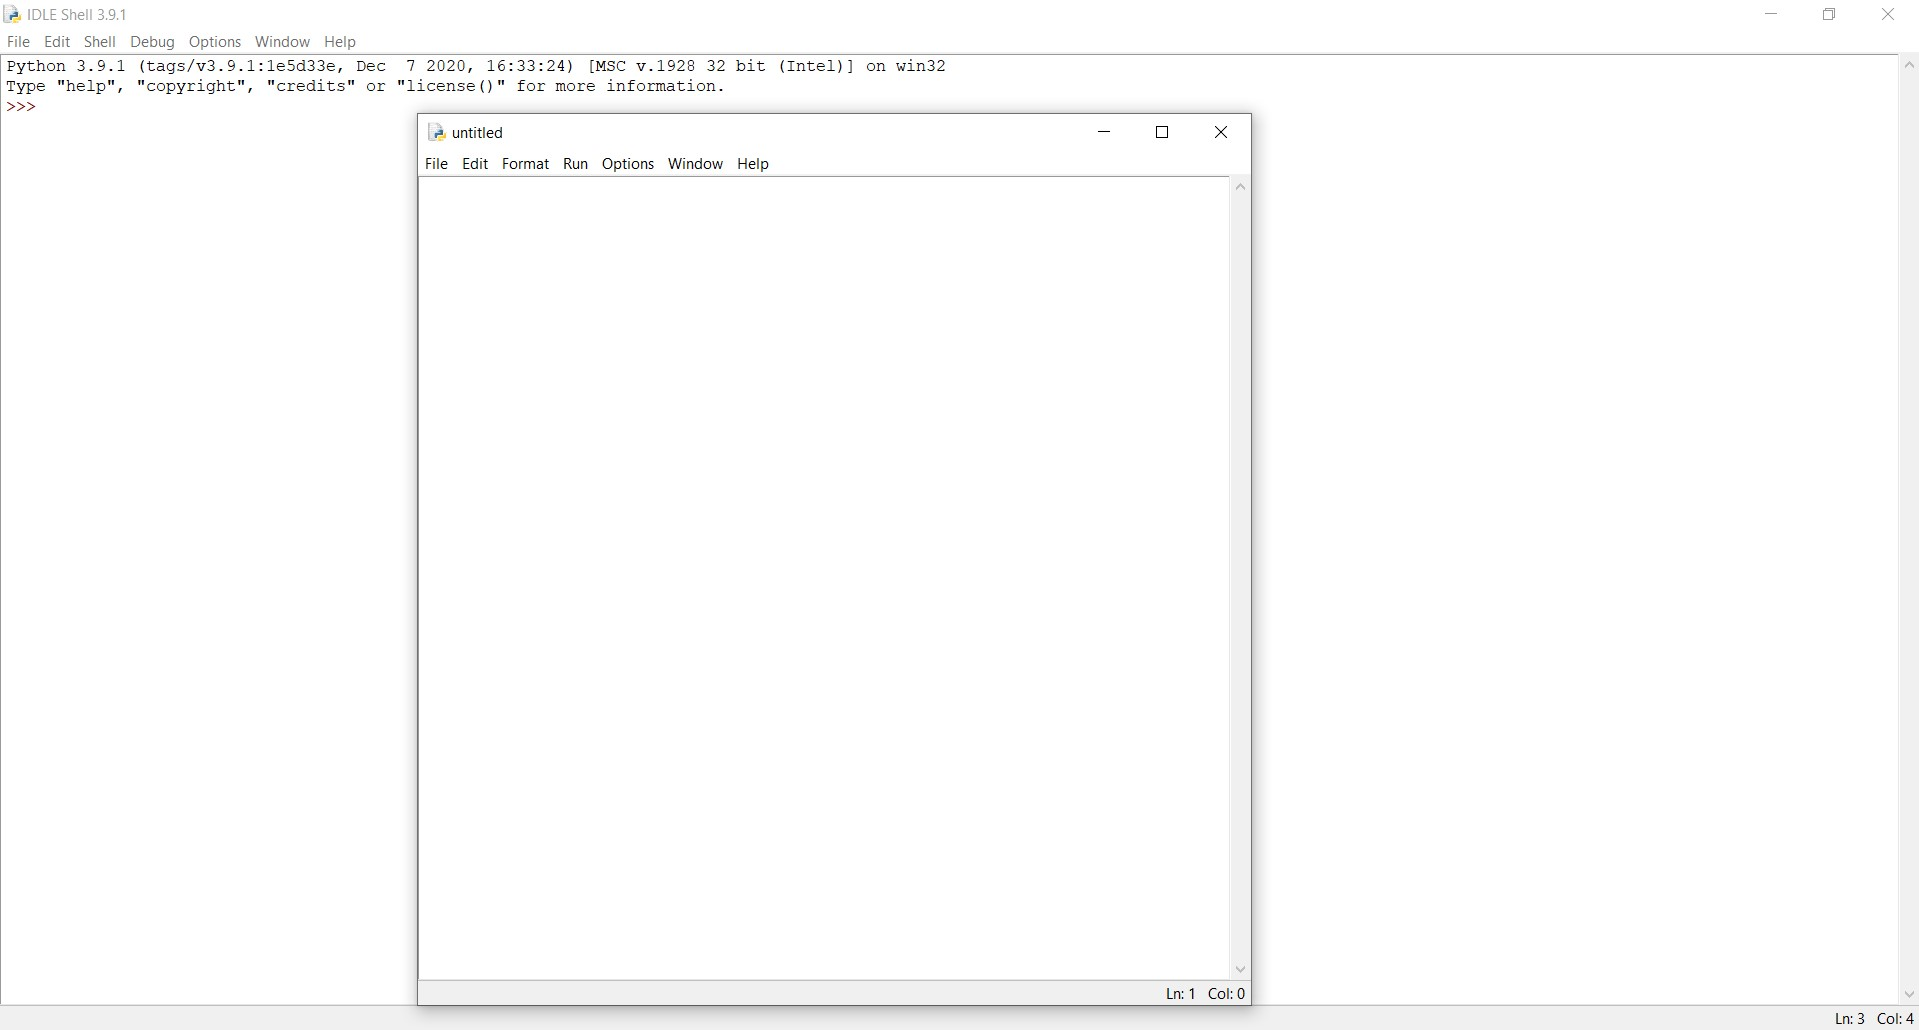
\includegraphics[width=1.0\textwidth]{slike/pythonIDLE.jpg}
    \caption{Python razvojno okruženje (Izvor: \citeauthor{idle}, \citeyear{idle})}
    \label{fig:PythonIDLE}
\end{figure}

\newpage

\chapter{Implementacija}

Kao što je i na početku ovog rada naznačeno tematika kojom ćemo se baviti je razvoj višeagentnog sustava koja će iz javno dostupnih resursa dohvaćati vijesti i prikazivati ih korisniku. Sustav se sastoji od jednog glavnog agenta, agenta za pretraživanje novosti na stranici Index.hr te agenta koji se bavi filtriranjem sadržaja.

Prije implementacije agenata potrebno je u programski kôd uključiti sve potrebne biblioteke za razvoj višeagentnog sustava na odabranu temu. Bibilioteke koje ćemo uključiti jesu \textit{spade}, \textit{beautifulsoup4}, \textit{requests}. Uključivanje u programski kôd prikazano je u sljedećem isječku:

\begin{lstlisting}[language=Python, caption={Potrebne biblioteke}]
import time

from spade.agent import Agent
from spade.behaviour import FSMBehaviour, State
from spade.message import Message

from bs4 import BeautifulSoup
import requests
\end{lstlisting}

\section{Implementacija agenta \textit{GlavniAgent}}
\textit{GlavniAgent} je glavni agent našeg višeagentnog sustava. Agent se sastoji od dva stanja: \textbf{PrvoStanje} i \textbf{DrugoStanje}. U stanju \textit{PrvoStanje} agent šalje agentu \textbf{RSSAgent} poruku da krenu s radom. U stanju \textit{DrugoStanje} agent čeka potvrdu da su novosti filtrirane te prikazuju novosti koje je korisnik zatražio. Agent po ispisivanju novosti završava s radom. Foramlizirani prikaz ovog agenta u skladu s definicijom za agente kao konačne automate izgledao bi kako slijedi:

\begin{itemize}
  \item \(\Sigma\) = $\{SaljiPoruku, CekajPoruku$\}
  \item \(\Gamma\) = $\{PorukaPoslana, PorukaPrimljena$\}
  \item \(S\) = $\{PrvoStanje, DrugoStanje$\}
  \item \(S_0\) = $\{PrvoStanje$\}
\end{itemize}

Nakon formaliziranog prikaza glavnog agenta slijedi isječak programskog kôda.
\begin{lstlisting}[language=Python, caption={Programski kôd za GlavniAgent agenta}]
STANJE_PRVO = "STANJE_PRVO"
STANJE_DRUGO = "STANJE_DRUGO"
STANJE_TRECE = "STANJE_TRECE"

class GlavniAgent(Agent):

    listaFiltriranihNovostiIndexHr = []
    class FSMPonasanje(FSMBehaviour):
        async def on_start(self):
            print(f"{GlavniAgent.__name__}: Pokrećem se ... ({self.current_state})")

        async def on_end(self):
            print(f"{GlavniAgent.__name__}: Završavam s radom ... {self.current_state}")
            await self.agent.stop()

    class StanjePrvo(State):
        async def run(self):
            print(f"{GlavniAgent.__name__}: Šaljem poruku za početak prikupljanje novosti s portala ...")
            msg = Message(to="vasprojekt2@jabber.eu.org")
            msg.body = "Započni s prikupljanjem novosti s portala!"
            await self.send(msg)
            print(f"{GlavniAgent.__name__}: Poruka poslana!")
            self.set_next_state(STANJE_DRUGO)

    class StanjeDrugo(State):
        async def run(self):
            print(f"{GlavniAgent.__name__}: Nalazim se u završnom stanju. Čekam na primitak poruke ...")
            msg = await self.receive(timeout=30)
            print(f"{GlavniAgent.__name__}: Poruka zaprimljena!")
                    
            if msg:
                if msg.body != '':
                    print(f"{GlavniAgent.__name__}: Zaprimio sam poruku sljedećeg sadržaja: \"{msg.body}\"")
                    print(f"{GlavniAgent.__name__}: Novosti prikupljene i spremne za prikaz.")
                    print("\n -------------------------------- \n")
                    print("\n --------- N O V O S T I -------- \n")
                    print("\n -------------------------------- \n")

                    counter = 1
                    for novost in GlavniAgent.listaFiltriranihNovostiIndexHr:
                        print(f"{counter}. {novost}")
                        counter += 1
                else:
                    print("Nema odgovora.")

    async def setup(self):
        agent = self.FSMPonasanje()
        agent.add_state(name=STANJE_PRVO, state=self.StanjePrvo(), initial=True)
        agent.add_state(name=STANJE_DRUGO, state=self.StanjeDrugo())
        agent.add_transition(source=STANJE_PRVO, dest=STANJE_DRUGO)
        self.add_behaviour(agent)
\end{lstlisting}

\section{Implementacija agenata \textit{RSSAgent}}
Kako bi mogli prikazivati novosti korisnicima sustava te novosti potrebno je prvo preuzeti s novinskih portala na internetu. Za to preuzimanje zadužen je agenti \textit{RSSAgent}. Kako i sam naziv govori agent će preuzimati novosti s portala Index.hr koje su na stranici pohranjene u RSS obliku. Riječ je o implementaciji koja se izvodi \textit{straightforward} a na  identičan način možemo implementirati bilo kojeg agenta samo ćemo umjesto u atribut \textit{addr} postaviti poveznicu na željeni RSS file.

Agenata \textit{RSSAgent} je agent koji se sastoji od tri stanja: \textbf{PrvoStanje}, \textbf{DrugoStanje} i \textbf{TreceStanje}. U stanju \textit{PrvoStanje} agent čeka da primi poruku od primarnog agenta za početak rada. U stanju \textit{DrugoStanje} agent preuzima novosti iz zadanog izvora i šalje ih agentu \textit{SearchAgent}. U stanju \textit{TreceStanje} agent šalje poruku da je gotov s preuzimanjem novosti agentu \textit{SearchAgent}.
Foramlizirani prikaz ovog agenta u skladu s definicijom za agente kao konačne automate izgledao bi kako slijedi:

\begin{itemize}
  \item \(\Sigma\) = $\{CekajPoruku, PreuzimanjeNovosti$\}
  \item \(\Gamma\) = $\{PorukaPrimljena, NovostiPreuzete$\}
  \item \(S\) = $\{PrvoStanje, DrugoStanje, TreceStanje$\}
  \item \(S_0\) = $\{PrvoStanje$\}
\end{itemize}

Nakon formaliziranog prikaza agenta slijedi isječak programskog kôda.
\begin{lstlisting}[language=Python, caption={Programski kôd za RSSAgent agenta}]
class RSSAgent(Agent):

    class FSMPonasanje(FSMBehaviour):
        async def on_start(self):
            print(f"{RSSAgent.__name__}: Pokrećem se ... ({self.current_state})")

        async def on_end(self):
            print(f"{RSSAgent.__name__}: Završavam s radom ... {self.current_state}")
            await self.agent.stop()

    class StanjePrvo(State):
        async def run(self):
            msg = await self.receive(timeout=15)
            print(f"{RSSAgent.__name__}: Zaprimio sam poruku sadržaja: \"{msg.body}\"")
            self.set_next_state(STANJE_DRUGO)

    class StanjeDrugo(State):
        async def run(self):
            listaAddr = []
            unos = ''
            while(unos != "\s"):
                unos = input("Unesi željeni RSS u obliku 'https://domain-name.xyz' (\"\\s\" - prekid unosa): ")
                if(unos != '\s'):
                    listaAddr.append(f"{unos}")
                else:
                    break
            for adresa in listaAddr:    
                addr = requests.get(f'{adresa}')
                nazivPortala = adresa.split("//")[1]
                RSSAgent = BeautifulSoup(addr.content, 'xml')
                items = RSSAgent.find_all('item')
                for item in items:
                    portal = nazivPortala
                    datum = item.pubDate.text
                    naslov = item.title.text
                    sazetak = item.description.text
                    poveznica = item.link.text
                    if(sazetak != ''):
                        SearchAgent.listaNovostiSPortala.append(f"\n\nPortal: {portal}\n\nDatum: {datum}.\n\nNaslov: {naslov}\n\nSažetak: {sazetak}\n\nPoveznica: {poveznica}\n\n----------------------------------")
                    else:
                        SearchAgent.listaNovostiSPortala.append(f"\n\nPortal: {portal}\n\nDatum: {datum}.\n\nNaslov: {naslov}\n\nPoveznica: {poveznica}\n\n----------------------------------")
            self.set_next_state(STANJE_TRECE)

    class StanjeTrece(State):
        async def run(self):
            print(f"{RSSAgent.__name__}: Šaljem poruku da sam završio s prikupljanjem novosti ...")
            msg = Message(to="vasprojekt3@jabber.eu.org")
            msg.body = "Završio s prikupljanjem novosti s portala!"
            await self.send(msg)
            print(f"{RSSAgent.__name__}: Poruka poslana!")

    async def setup(self):
        agent = self.FSMPonasanje()
        agent.add_state(name=STANJE_PRVO, state=self.StanjePrvo(), initial=True)
        agent.add_state(name=STANJE_DRUGO, state=self.StanjeDrugo())
        agent.add_state(name=STANJE_TRECE, state=self.StanjeTrece())
        agent.add_transition(source=STANJE_PRVO, dest=STANJE_DRUGO)
        agent.add_transition(source=STANJE_DRUGO, dest=STANJE_TRECE)
        self.add_behaviour(agent)
\end{lstlisting}
\section{Implementacija agenta \textit{SearchAgent}}
Agent \textit{SearchAgent} kao što mu i samo ime kaže služi za pretraživanje odnosno filtraciju novosti koje su preuzete s agentom \textit{RSSAgent}. Svrha ovog agenta očituje se u funkciji filtriranja novosti relevantnih traženom pojmu. Kao i ostali agenti u ovom sustavu i ovaj se na početku inicijalizira u sustavu i postavlja u stanje čekanja. Sastoji se od tri stanja: \textbf{PrvoStanje}, \textbf{DrugoStanje} i \textbf{TreceStanje}. Stanje čekanja je stanje \textbf{PrvoStanje}. Nakon što agent završi s preuzimanjem novosti prelazi u stanje \textbf{TreceStanje} gdje se šalje zahtjev agentu \textit{SearchAgent} za pretraživanje novosti po unesenom pojmu. Nakon što je stanje \textbf{PrvoStanje} primilo poruku da je agent \textit{RSSAgent} završio s prikupljanjem novosti agent \textit{SearchAgent} prelazi u stanje \textbf{DrugoStanje} gdje prima korisnički unos za pretraživanje po određenom pojmu. Kada pretraživanje završi, a vijesti s tim pojmom budu prikupljene agent \textit{SearchAgent} prelazi u stanje \textbf{TreceStanje} i šalje poruku agentu \textit{GlavniAgent} da je gotov. Sada agent \textit{GlavniAgent} ispisuje pretražene novosti. Nakon ispisa višeagentni sustav završava s radom. 

Foramlizirani prikaz ovog agenta u skladu s definicijom za agente kao konačne automate izgledao bi kako slijedi:

\begin{itemize}
  \item \(\Sigma\) = $\{CekajPoruku, FiltriranjeNovosti, SaljiPoruku$\}
  \item \(\Gamma\) = $\{PorukaPrimljena, NovostiFiltrirane$\}
  \item \(S\) = $\{PrvoStanje, DrugoStanje, TreceStanje$\}
  \item \(S_0\) = $\{PrvoStanje$\}
\end{itemize}

Nakon formaliziranog prikaza  agenta slijedi isječak programskog kôda filtracije.

\begin{lstlisting}[language=Python, caption={Programski kôd za SearchAgent agenta}]
class SearchAgent(Agent):


    listaNovostiIndexHr = []
    class FSMPonasanje(FSMBehaviour):
        async def on_start(self):
            print(f"{SearchAgent.__name__}: Pokrećem se ... ({self.current_state})")

        async def on_end(self):
            print(f"{SearchAgent.__name__}: Završavam s radom ... {self.current_state}")
            await self.agent.stop()

    class StanjePrvo(State):
        async def run(self):
            msg = await self.receive(timeout=15)
            print(f"{SearchAgent.__name__}: Zaprimio sam poruku sadržaja: \"{msg.body}\"")
            self.set_next_state(STANJE_DRUGO)
            
    class StanjeDrugo(State):
        async def run(self):
            
            unos = input("Unesi pojam za pretraživanje (\"all\" - prikaz svih vijesti): ")

            if (unos != "all"):
                for novost in SearchAgent.listaNovostiIndexHr:
                    if(unos in novost):
                        GlavniAgent.listaFiltriranihNovostiIndexHr.append(novost)
                print("Vijesti su filtrirane!")
                self.set_next_state(STANJE_TRECE)
            else:
                for novost in SearchAgent.listaNovostiIndexHr:
                    GlavniAgent.listaFiltriranihNovostiIndexHr.append(f"{novost}")
                    self.set_next_state(STANJE_TRECE)


    class StanjeTrece(State):
        async def run(self):
            print(f"{SearchAgent.__name__}: Šaljem poruku da sam završio s filtriranjem novosti ...")
            msg = Message(to="vasprojekt1@jabber.eu.org")
            msg.body = "Završio s filtracijom novosti s portala!"
            await self.send(msg)
            print(f"{SearchAgent.__name__}: Poruka poslana!")   

    async def setup(self):
        agent = self.FSMPonasanje()
        agent.add_state(name=STANJE_PRVO, state=self.StanjePrvo(), initial=True)
        agent.add_state(name=STANJE_DRUGO, state=self.StanjeDrugo())
        agent.add_state(name=STANJE_TRECE, state=self.StanjeTrece())
        agent.add_transition(source=STANJE_PRVO, dest=STANJE_DRUGO)
        agent.add_transition(source=STANJE_DRUGO, dest=STANJE_TRECE)
        agent.add_transition(source=STANJE_DRUGO, dest=STANJE_TRECE)
        self.add_behaviour(agent)
\end{lstlisting}

\chapter{Zaključak}

U ovom projektu za zadatak je bilo implementirati višeagentni sustav za preuzimmanje, filtriranje i prikazivenje novosti koristeći SPADE i  Python. Tema je bila osobni izbor svakog studenta dakle proizvoljna ali u skladu s akademskim okruženjem. Očekivanja koja sam imao od teme  na početku izrade bila jako niska jer sama svijest da pristupam radu s Python programskim jezikom mi je bila zastrašujuća. Kako je projekt išao k svome vrhuncu nadao sam se da ću negdje u dubini svoje duše zavoljeti rad u Pythonu ali to se nije dogodilo. Uz pisanje dokumentacije u \LaTeX -u sintaksa programskog jezika Python i biblioteke koje prvi put koristim su mi bili najveći izazovi ovog projekta.

Osim na kolegiju Višeagentni sustavi do sada nisam imao prilike se susresti ovako opsežno s Python programskim jezikom tako da sam sada imao mnoge prepreke koje sam morao savladati kako bi uspješno realizirao projekt.

U samoj konačnici realizirao sam mali višeagentni sustav za prikupljanje novosti. Smatram ovaj sustav dobrim početkom. Na sustavu bi se moglo još poraditi u smislu da se nadopuni još dodatnim agentima na određene stranice. Filtriranje informacija bi moglo biti malo bolje realizirano. Sustav bi mogao nadopuniti da preuzima cijele vijesti ali to bi zahtjevalo malo veću doradu. Sve u svemu zadovoljan sam rezultatom iako se moglo više i bolje.

\makebackmatter
% generira popis korištene literature, popis slika (ako je primjenjivo), popis tablica (ako je primjenjivo) i popis isječaka koda (ako je primjenjivo)

%\appendices % ako nije potrebno, obrisati ili zakomentirati

%\chapter{Prilog 1} % ako nije potrebno, obrisati ili zakomentirati

%\chapter{Prilog 2} % ako nije potrebno, obrisati ili zakomentirati

\end{document}
